%% abtex2-modelo-trabalho-academico.tex, v-1.9.2 laurocesar
%% Copyright 2012-2014 by abnTeX2 group at http://abntex2.googlecode.com/ 
%%
%% This work may be distributed and/or modified under the
%% conditions of the LaTeX Project Public License, either version 1.3
%% of this license or (at your option) any later version.
%% The latest version of this license is in
%%   http://www.latex-project.org/lppl.txt
%% and version 1.3 or later is part of all distributions of LaTeX
%% version 2005/12/01 or later.
%%
%% This work has the LPPL maintenance status `maintained'.
%% 
%% The Current Maintainer of this work is the abnTeX2 team, led
%% by Lauro César Araujo. Further information are available on 
%% http://abntex2.googlecode.com/
%%
%% This work consists of the files abntex2-modelo-trabalho-academico.tex,
%% abntex2-modelo-include-comandos and abntex2-modelo-references.bib
%%

% ------------------------------------------------------------------------
% ------------------------------------------------------------------------
% abnTeX2: Modelo de Trabalho Academico (tese de doutorado, dissertacao de
% mestrado e trabalhos monograficos em geral) em conformidade com 
% ABNT NBR 14724:2011: Informacao e documentacao - Trabalhos academicos -
% Apresentacao
% ------------------------------------------------------------------------
% ------------------------------------------------------------------------

\documentclass[
	% -- opções da classe memoir --
	12pt,				% tamanho da fonte
	openright,			% capítulos começam em pág ímpar (insere página vazia caso preciso)
	twoside,			% para impressão em verso e anverso. Oposto a oneside
	a4paper,			% tamanho do papel. 
	% -- opções da classe abntex2 --
	%chapter=TITLE,		% títulos de capítulos convertidos em letras maiúsculas
	%section=TITLE,		% títulos de seções convertidos em letras maiúsculas
	%subsection=TITLE,	% títulos de subseções convertidos em letras maiúsculas
	%subsubsection=TITLE,% títulos de subsubseções convertidos em letras maiúsculas
	% -- opções do pacote babel --
	english,			% idioma adicional para hifenização
	french,				% idioma adicional para hifenização
	spanish,			% idioma adicional para hifenização
	brazil				% o último idioma é o principal do documento
	]{abntex2}

% ---
% Pacotes básicos 
% ---
\usepackage{lmodern}			% Usa a fonte Latin Modern			
\usepackage[T1]{fontenc}		% Selecao de codigos de fonte.
\usepackage[utf8]{inputenc}		% Codificacao do documento (conversão automática dos acentos)
\usepackage{lastpage}			% Usado pela Ficha catalográfica
\usepackage{indentfirst}		% Indenta o primeiro parágrafo de cada seção.
\usepackage{color}				% Controle das cores
\usepackage{graphicx}			% Inclusão de gráficos
\usepackage{microtype} 			% para melhorias de justificação
% ---
		
% ---
% Pacotes adicionais, usados apenas no âmbito do Modelo Canônico do abnteX2
% ---
\usepackage{lipsum}				% para geração de dummy text
% ---

% ---
% Pacotes de citações
% ---
\usepackage[brazilian,hyperpageref]{backref}	 % Paginas com as citações na bibl
\usepackage[alf]{abntex2cite}	% Citações padrão ABNT

% --- 
% CONFIGURAÇÕES DE PACOTES
% --- 

% ---
% Configurações do pacote backref
% Usado sem a opção hyperpageref de backref
\renewcommand{\backrefpagesname}{Citado na(s) página(s):~}
% Texto padrão antes do número das páginas
\renewcommand{\backref}{}
% Define os textos da citação
\renewcommand*{\backrefalt}[4]{
	\ifcase #1 %
		Nenhuma citação no texto.%
	\or
		Citado na página #2.%
	\else
		Citado #1 vezes nas páginas #2.%
	\fi}%
% ---

% ---
% Informações de dados para CAPA e FOLHA DE ROSTO
% ---
\titulo{Modelagem Matemática da Malária}
\autor{Emanuel Bissiatti de Almeida \\ Rafael Gomes Portácio de Souza}
\local{Brasil}
\data{2021}
\orientador{Flávio Codeço Coelho}
\instituicao{%
  Fundação Getúlio Vargas -- FGV
  \par
  Escola de Matemática Aplicada -- EMAp
  \par
  }
\tipotrabalho{Trabalho de Modelagem Biológica}
% O preambulo deve conter o tipo do trabalho, o objetivo, 
% o nome da instituição e a área de concentração 
\preambulo{Modelagem matemática de disseminação epidemiológica da malária.}
% ---


% ---
% Configurações de aparência do PDF final

% alterando o aspecto da cor azul
\definecolor{blue}{RGB}{41,5,195}

% informações do PDF
\makeatletter
\hypersetup{
     	%pagebackref=true,
		pdftitle={\@title}, 
		pdfauthor={\@author},
    	pdfsubject={\imprimirpreambulo},
	    pdfcreator={LaTeX with abnTeX2},
		pdfkeywords={abnt}{latex}{abntex}{abntex2}{trabalho acadêmico}, 
		colorlinks=true,       		% false: boxed links; true: colored links
    	linkcolor=blue,          	% color of internal links
    	citecolor=blue,        		% color of links to bibliography
    	filecolor=magenta,      		% color of file links
		urlcolor=blue,
		bookmarksdepth=4
}
\makeatother
% --- 

% --- 
% Espaçamentos entre linhas e parágrafos 
% --- 

% O tamanho do parágrafo é dado por:
\setlength{\parindent}{1.3cm}

% Controle do espaçamento entre um parágrafo e outro:
\setlength{\parskip}{0.2cm}  % tente também \onelineskip

% ---
% compila o indice
% ---
\makeindex
% ---

% ----
% Início do documento
% ----
\begin{document}

% Retira espaço extra obsoleto entre as frases.
\frenchspacing 

% ----------------------------------------------------------
% ELEMENTOS PRÉ-TEXTUAIS
% ----------------------------------------------------------
% \pretextual

% ---
% Capa
% ---
\imprimircapa
% ---

% ---
% Folha de rosto
% (o * indica que haverá a ficha bibliográfica)
% ---
\imprimirfolhaderosto*
% ---

% ---
% Inserir a ficha bibliografica
% ---

% Isto é um exemplo de Ficha Catalográfica, ou ``Dados internacionais de
% catalogação-na-publicação''. Você pode utilizar este modelo como referência. 
% Porém, provavelmente a biblioteca da sua universidade lhe fornecerá um PDF
% com a ficha catalográfica definitiva após a defesa do trabalho. Quando estiver
% com o documento, salve-o como PDF no diretório do seu projeto e substitua todo
% o conteúdo de implementação deste arquivo pelo comando abaixo:
%
% \begin{fichacatalografica}
%     \includepdf{fig_ficha_catalografica.pdf}
% \end{fichacatalografica}

\newpage

% ---
% inserir o sumario
% ---
\pdfbookmark[0]{\contentsname}{toc}
\tableofcontents*
\cleardoublepage
% ---



% ----------------------------------------------------------
% ELEMENTOS TEXTUAIS
% ----------------------------------------------------------
\textual

% ----------------------------------------------------------
% Introdução (exemplo de capítulo sem numeração, mas presente no Sumário)
% ----------------------------------------------------------
\chapter*[Introdução]{Introdução}
\addcontentsline{toc}{chapter}{Introdução}
% ----------------------------------------------------------

\\
A malária é uma doença não contagiosa que é transmitida por mosquitos fêmeas do gênero  \textit{Anopheles} \footnote{mosquitos de gênero também são conhecidos como mosquito-prego.} portadoras do protozoário \textit{Plasmodium}. Esse inseto é típico de climas úmidos e quentes. No Brasil, existe uma concentração dos mosquitos - e dos casos da doença -  na região Amazônica.

Essa doença normalmente apresenta sintomas de febre alta, dores de cabeça, temores, calafrios e em alguns casos pode apresentar dores no corpo, perda do apetite, cansaço, vômitos e diarreia. Felizmente, segundo o Ministério da Saúde, a letalidade da malária é baixa: na região Amazônica é de 1,6/100.000 \cite{SUS} enquanto no restante do país a letalidade é cerca de 128 vezes maior. Isso ocorre, pois, o tratamento da malária disponibilizado pelo Ministério da Saúde,  principalmente na região Amazônica, é eficiente. Já nas outras regiões onde a malária é rara, a doença é mais difícil de ser identificada, e portanto possuiu tratamento menos eficaz.    


Esse inseto põe ovos em locais de água parada, sendo assim, a densidade de mosquitos tende a aumentar conforme maior for a umidade do local. Por outro lado, outro fator climático que também interfere em sua proliferação, é o fato de que as fortes chuvas podem arrastar tais ovos(ou larvas) e diminuir assim a futura população desses mosquitos. Devido a tais fatores e ao seu curto ciclo de vida, a população desses insetos é extremamente dependente das condições climáticas e por causa disso é interessante que modelos que não consideram a interferência temporal sejam aplicados para pequenos espaços de tempo.

Pessoas que já foram infectadas múltiplas vezes pela malária só apresentam imunidade parcial assim como não há uma vacina para a doença. Devido a isso, o foco de sua contenção está principalmente nas outras medidas de prevenção. Visando prever os níveis de disseminação dessa doença, esse trabalho faz uma modelagem epidemiológica, isto é, neste caso, uma análise em função do tempo do comportamento populacional do vetor da malária bem como a taxa de infectados da população humana.

O primeiro modelo matemático da disseminação da Malária proposto foi o modelo de Ross-McDonald \cite{ndacherenga2019modelos}, em que é adotado um modelo SIS para o comportamento da população humana e SI para a população de mosquitos, que não se recuperam. O modelo porém assume que ambas as populações tem quantidade total constante. Suposição essa que não condiz com a realidade da população do mosquito uma vez que ela é fortemente influenciada por diversos fatores e também possui um curtíssimo ciclo de vida, o que favorece rápidas mudanças na população. Para medir as taxas de infecção nessas duas populações, o modelo assume que a taxa de infecção de uma população é proporcional à quantidade de indivíduos suscetíveis dela e também à quantidade de indivíduos da outra população que estejam infectados.


Já o modelo alternativo proposto em \cite{macufa} apresenta uma modelagem visando a simplificação de dimensões. Por isso, o autor decidiu desconsiderar a dinâmica de populações entre os humanos e os mosquitos. Nele, diferente do Ross-McDonald, a taxa de contaminação é proporcional a quantidade de infectados multiplicado pela constante relacionada a densidade de mosquitos na região. Dessa forma, o modelo proposto apresenta 3 equações baseadas no modelo SIR. Ressaltamos que, no caso da malária, após sair do estado de infectado apenas uma pequena fração da população permanece recuperada, enquanto a grande maioria retorna ao grupo de suscetíveis.


No modelo em \cite{wyse2006modelo} adota-se um modelo SEIS para população humana e SEI para a dos mosquitos que fazem parte do grupo de possíveis vetores (fêmeas em fase adulta). Nele assume-se apenas a população humana como constante: as taxas de natalidade e mortalidade que estão inclusas no modelo são iguais. Já a população de mosquitos segue o crescimento logístico, pois o seu ciclo de vida é curto quando comparado aos humanos. Semelhante ao modelo de Ross-McDonald, as taxas de contato com a doença, que nesse caso representam a transição de suscetível para exposto, são proporcionais ao produto da respectiva população suscetível com a população infectada da outra espécie. O modelo também considera a existência de múltiplas formas de tratamento, cada uma com um diferente grau de eficácia.

Dessa forma, é relevante que haja modelos de predição para que se saibam as zonas mais prováveis de disseminação, por isso, usaremos para a população humana o modelo SIS (Suscetíveis Infectados Suscetíveis) e SI para o mosquito. Assumindo que apenas a população humana é constante. 



\chapter*[Metodologia]{Metodologia}
\addcontentsline{toc}{chapter}{Metodologia}

Em nossa análise, vamos modelar o vetor como a população de mosquitos fêmeas do gênero \textit{Anopheles}, mais comum transmissor da malária no Brasil, e a população humana que vive na região amazônica onde se localiza a maior quantidade de casos de malária no país. No nosso modelo, a população de mosquito $V$ segue um crescimento proporcional à população em relação ao tempo enquanto a população $H$ permanece constante. Essa decisão se justifica no ciclo de vida curto do mosquito quando comparado ao do homem e na baixa mortalidade da doença na região Amazônica. Temos:

$\frac{\partial H}{\partial t} = 0 $ 

$ \frac{\partial V}{\partial t}= \frac{nV(k-V)}{k} -mV$

(Onde ambos $H$ e $V$ são medidos nas respectivas unidades populacionais $U.H.$ e $U.V.$. Exemplos comuns de unidades populacionais: milhares de indivíduos, milhões de indivíduos.)

Com relação da doença, vamos descrever a população humanos com o modelo SIS (Suscetível-Infectado-Suscetível), já que a malária é uma doença causa por protozoários: sua imunidade é baixa e a reinfecção por malária é comum no país \cite{SUS}. No caso do vetor, temos um modelo SI (Suscetível-Infectado), por simplicidade, consideramos que todos os mosquitos fêmeas nascem suscetíveis a doença e quando picam algum humano contaminado passam ao estado de infectado, quando já contamina os humanos ao sugar o seu sangue. Seja:

\begin{itemize}
    \item $t$ a unidade de tempo
    \item $H_S$ quantidade de humanos suscetíveis;
    \item $H_I$ quantidade de humanos infectados;
    \item $V_S$ quantidade de mosquitos suscetíveis;
    \item $V_I$ quantidade de mosquitos infectados;
    \item $c$ é um fator para converter uma quantidade que está na unidade $U.H.$ para $U.V.$ (unid: $U.H.^{-1}U.V.$);
    \item $a,b,p,q,n,m,k$ constantes;
    \item $a$ é a taxa de humanos picados por uma unidade de mosquito por unidade tempo (unid: $U.H.\cdot U.V.^{-1}T^{-1}$);
    \item $b$ é a taxa de recuperação dos humanos por unidade tempo (unid: $T^{-1}$);
    \item $p$ é a probabilidade de uma picada infectar um humano;
    \item $q$ é a probabilidade de uma picada infectar um mosquito;
    \item $n$ é a taxa de natalidade dos mosquitos, por hipótese, todo mosquito nasce suscetível (unid: $T^{-1}$);
    \item $m$ é a taxa de mortalidade dos mosquitos (unid: $T^{-1}$);
    \item $k$ é a constante limite do modelo logístico  (unid: $T^{-1}$). 
\end{itemize}

Considerando o modelo SIS para humanos e SI para mosquitos temos as equações:

$H = H_I+H_S$
 

$V = V_I + V_S$

De acordo com essas equações, apenas com a quantidade de infectados e tamanho da população é possível descobrir o número de suscetíveis. Então, a variação populacional em relação ao tempo será:

\textbf{Para a população humana:}

$$ \frac{\partial H_I}{\partial t}= a pV_I\frac{(H-H_I)}{H}- b H_I$$

Onde a parcela $a pV_I\frac{H-H_I}{H}$ representa a taxa de infecção, seguindo a ideia de que $a\cdot V_I$ é a taxa total de humanos picados por mosquitos infectados por unidade de tempo. Então ao multiplicar isso pela probabilidade $p$ da picada infectar o humano, teremos a taxa de infecções em humanos por unidade de tempo. Porém a infecção só é relevante para quem é suscetível, então ao multiplicar por $\frac{H_S}{H}$ (ou $\frac{(H-H_I)}{H}$) teremos a taxa de infecção nos humanos suscetíveis.
A parcela $-b H_I$ representa a recuperação dos humanos do estado de infectado. (Note que $\frac{\partial H_I}{\partial t}=-\frac{\partial H_S}{\partial t}$)

\textbf{Para a população dos vetores:}

$$ \frac{\partial V_I}{\partial t}= \Big(a(V-V_I)\frac{H_I}{H}\Big)cq-m V_I$$

$$ \frac{\partial V_S}{\partial t}= n\frac{k-V}{k}V-\Big(aV_S\frac{H_I}{H}\Big)cq-m V_S$$

Onde a parcela $\Big(a(V-V_I)\frac{H_I}{H}\Big)cq$ representa a taxa de infecção seguindo uma ideia semelhante à da população humana. $a(V-V_I)$ é a taxa total de humanos picados por mosquitos suscetíveis, multiplicando pela razão $\frac{H_I}{H}$ teremos a taxa de humanos infectados picados por mosquitos suscetíveis, note que essa é a taxa de eventos de possível infecção medida na unidade de $U.H.\cdot T^{-1}$, multipliquemos por um fator de conversão para a termos em $U.V.\cdot T^{-1}$ e então multipliquemos por $q$ para termos então a taxa de infecção nos mosquitos. A parcela $nV$ representa a natalidade. As parcelas $mV_I$ e $mV_S$ representam respectivamente a mortalidade dos suscetíveis e dos infectados.

Observe que estamos trabalhando com três grandezas lineares nesse sistema, o número de indivíduos da população humana, o número de indivíduos da população de fêmeas do mosquito e o tempo. As equações, por sua vez referem-se a variação da quantidade de indivíduos em função do tempo. Fazendo a análise dimensional das equações, vemos que todas estão dimensionadas corretamente:
$$ \frac{\partial H_I}{\partial t}= a pV_I\frac{(H-H_I)}{H}- b H_I$$
$$U.H.\cdot T^{-1}=\frac{U.H.}{U.V.\cdot T}\cdot 1\cdot U.V.\frac{U.H.}{U.H.} - T^{-1}U.H.$$
$$U.H.\cdot T^{-1}=U.H.\cdot T^{-1}$$


$$ \frac{\partial V_I}{\partial t}= \Big(a(V-V_I)\frac{H_I}{H}\Big)cq-m V_I$$
$$U.V.\cdot T^{-1}=\Big(\frac{U.H.}{U.V.\cdot T} (U.V.-U.V.)\frac{U.H.}{U.H.}\Big)\frac{U.V.}{U.H.}\cdot 1 - T^{-1}U.V.$$
$$U.V.\cdot T^{-1}=U.V.\cdot T^{-1}$$


$$ \frac{\partial V_S}{\partial t}= n\frac{k-V}{k}V-\Big(aV_S\frac{H_I}{H}\Big)cq-m V_S$$
$$U.V.\cdot T^{-1} = T^{-1}\frac{U.V.}{U.V.}U.V. -  \Big(\frac{U.H.}{U.V.\cdot T} (U.V.-U.V.)\frac{U.H.}{U.H.}\Big)\frac{U.V.}{U.H.}\cdot 1 - T^{-1}U.V.$$
$$U.V.\cdot T^{-1}=U.V.\cdot T^{-1}$$

\chapter*[Resultado]{Resultado}
\addcontentsline{toc}{chapter}{Resultado}
No equilíbrio da população humana:
$$ 0= a pV_I^\ast\frac{(H-H_I^\ast)}{H}- b H_I^\ast$$
$$a pV_I^\ast\frac{H_S^\ast}{H}= b H_I^\ast$$
$$\frac{a pV_I^\ast}{bH}= \frac{H_I^\ast}{H_S^\ast}$$
Ou seja:
$$H_I^\ast = \frac{HapV_I^\ast}{\Big(bH+apV_I^\ast\Big)}$$
$$H_S^\ast = \frac{H^2b}{\Big(bH+apV_I^\ast\Big)}$$

No equilíbrio da população de insetos infectados:
$$\Big(a(V^\ast-V_I^\ast)\frac{H_I^\ast}{H}\Big)cq=m V_I^\ast$$
$$\Big(a(V_S^\ast)\frac{H_I^\ast}{H}\Big)cq=m V_I^\ast$$
$$\frac{mH}{aH_I^\ast cq}=\frac{V_S^\ast}{V_I^\ast}$$

Podemos manipular as equações acima para obter a equação abaixo:

$$\frac{m(bH + apV^\ast_I)}{a^2p cq}=V_S^\ast$$

A seguir temos o equilíbrio da população de insetos total:
$$n\frac{k-V^\ast}{k}V^\ast-m V^\ast=0$$
$$n\frac{k-V^\ast_I - V^\ast_S}{k}(V^\ast_I + V^\ast_S)- m V^\ast=0$$
Seja a população diferente de zero, então:
$$V^\ast=\frac{(n-m)}{n}k$$
Note que para $n<m$ então a população decrescerá sempre, não importando as condições, então suponhamos $n\ge m.$
Voltando para a equação que tínhamos antes, podemos concluir que:
$$\frac{m(bH + apV^\ast_I)}{a^2p cq}=V^\ast - V_I^\ast$$
$$\frac{m(bH + apV^\ast_I)}{a^2p cq}=\frac{(n-m)}{n}k - V_I^\ast$$
Após algumas manipulações:
$$V^\ast_I=\frac{a^2p cq\frac{(n-m)}{n}k-mbH}{apm+a^2p cq}$$
E então:
$$V^\ast_S=\frac{ap m\frac{(n-m)}{n}k+mbH}{apm+a^2p cq}$$
$$H_I^\ast = \frac{H(a^2pcq\frac{(n-m)}{n}k-mbH)}{a^2pcq\frac{(n-m)}{n}k+acqbH}$$
$$H_S^\ast = \frac{bH^2(acq+m)}{a^2pcq\frac{(n-m)}{n}k+acqbH}$$

Note então que $H^\ast_I$, $H^\ast_S$, $V_I^\ast$ e $V_S^\ast$ serão equilibrados de forma estável desde que tenhamos $a^2p cq\frac{(n-m)}{n}k\ge mbH$, caso o contrário os equilíbrios $H^\ast_I$ e $V^\ast_I$ terão valor negativo. O equilíbrio $H^\ast_S$ terá valor acima de $H$. E o equilíbrio $V_S^\ast$ será maior que o equilíbrio $V^\ast.$\\

Observe que quando ocorre a seguinte igualdade teremos um igual equilíbrio entre os humanos saudáveis e infectados: $$H(a^2pcq\frac{(n-m)}{n}k-mbH)=bH^2(acq+m)$$

Escolhendo constantes de forma que ocorra essa igualdade entre ambas as populações, testemos em nossa simulação:


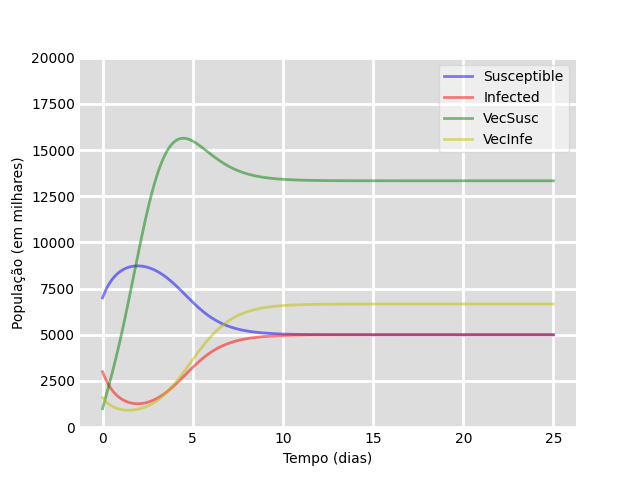
\includegraphics[width=410px]{Figure_1.png}

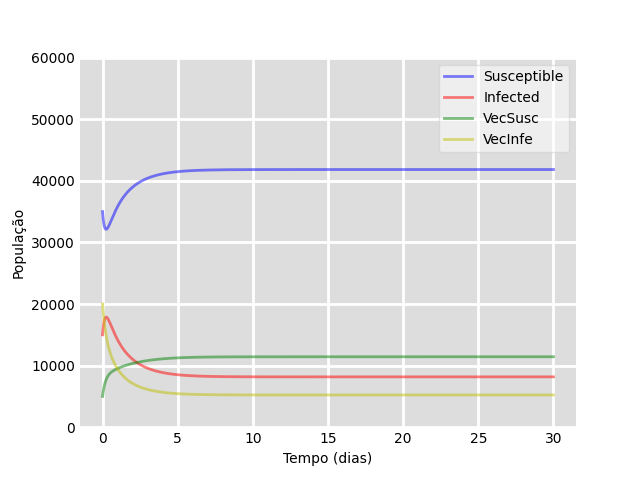
\includegraphics[width=410px]{Figure_6.png}

Para a próxima simulação, nós alteramos o modelo ao considerar o limite $k$ do modelo não como uma constante, mas sim como uma função cosseno do tempo, limitada entre em alguns valores:

\begin{itemize}
    \item Seja $dia0$ o dia do ano onde o ambiente é menos propenso para a reprodução dos mosquitos.
    
    \item Seja $kmax$ o valor máximo assumido por $k$ durante o ano
    
    \item Seja $kmin$ o valor mínimo assumido por $k$ durante o ano.
    
    \item considere $t$ o tempo em dias.
    
\end{itemize}
Então a função que descreve $k$

    $y = \pi + (x-dia0)\frac{2\pi}{365}$
    
    $k(t) = (kmax + kmin + (kmax-kmin)\cos(y))/2$

Tomamos essa decisão para melhor representar a realidade no modelo quando simulamos um longo período de tempo. 


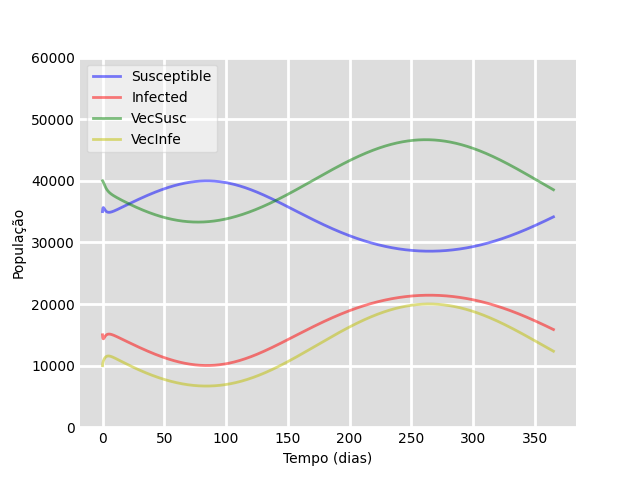
\includegraphics[width=410px]{Figure_10.png}

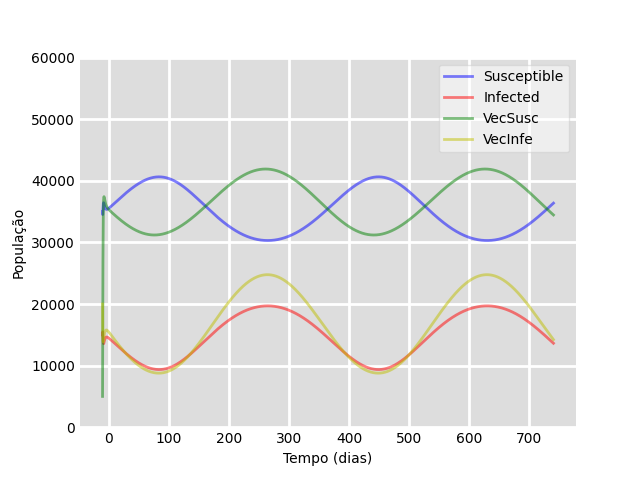
\includegraphics[width=410px]{Figure_4.png}

Por fim, uma simulação em que a doença não se desenvolve na população\\.

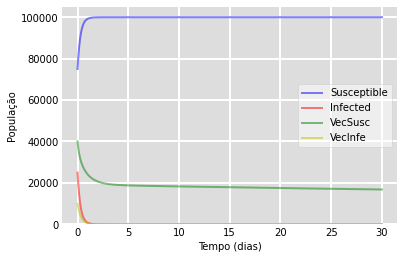
\includegraphics[width=410px]{output.png}

\chapter*[Discussão dos resultados]{Discussão dos resultados}




Observe que, em pequeno espaço de tempo $t$ em dias, em nossas simulações com constantes definidas aleatoriamente, o modelo se estabiliza. De fato esse comportamento era esperado desde a construção do modelo: consideramos a população humana permanecendo constante no período de tempo e a população do vetor cresce seguindo um modelo logístico, então foi possível concluir que, pelas equações, haveria um ponto de equilíbrio. Assim, esse modelo é pensado para descrever o início de um surto da malária, afim de previr que este possa ocorrer. 

No modelo aqui trabalhado, podemos traçar estimativas para o curto prazo e analisar múltiplos cenários ao se modificar as variáveis desejadas. Pelos equilíbrios, podemos analisar a desigualdade que precisa ser satisfeita para que a doença se sustente em nosso modelo ($a^2p cq\frac{(n-m)}{n}k\ge mbH$). Caso essa desigualdade não seja obedecida, segundo o nosso modelo, a doença naturalmente sumiria e deixaria de ser um problema.


Ressaltamos que o crescimento populacional dos mosquitos se dá em um determinado período do ano, no início da temporada de chuvas, e meses depois a população decresce. Sendo assim, é de se esperar que este modelo não condiz com a realidade em um logo período de tempo, porém, suficiente para entender o comportamento da doença em pequeno espaço de tempo.

Então, com o objetivo de adequar o modelo a realidade brasileira - a malária como uma doença que afeta os moradores da região amazônia anualmente principalmente na primavera \cite{boletim} - propomos que a taxa $k$ limitante do modelo logístico para a natalidade da população de mosquitos
seguisse uma função $cosseno$ em uma escala anual, para que pudéssemos simular a malária como uma doença sazonal. 

Apesar de obtermos algumas informações sobre o comportamento anual da malária, é evidente que não se trata de um retrato fiel da realidade brasileira. Os dados da malária ainda são escassos, e nós desconhecemos as populações das cidades onde foram estes foram registrados bem como o número de vetores presentes na região. 

Sendo assim, deixamos aqui registrado apenas uma sugestão para uma análise sazonal da malária com o objetivo de estudar a interferência da variação da população dos mosquitos no número de casos da malária. Dessa pequena análise, observamos que quanto maior a população total de mosquitos, maior o número de infectados, fato que é observado na equação:  $ \frac{\partial V_S}{\partial t}= n\frac{k-V}{k}V-\Big(aV_S\frac{H_I}{H}\Big)cq-m V_S$




\chapter*[Conclusão]{Conclusão}

A malária mesmo que causando poucas mortes no país afeta anualmente milhares de brasileiros na região amazônica. Infelizmente, a ciência ainda não descobriu uma vacina para a malária, além de que, por ser uma doença causada por um protozoário, a resposta imune natural do corpo humano é baixa. Sendo assim, é importante compreender o comportamento tanto do vetor, quanto da população em relação a doença, para que os agentes públicos possam combater com mais eficiência a doença.


Semelhante ao Ross-MacDonald, nosso modelo considera as taxas de infecção proporcionais às populações suscetíveis, sendo porém mais próximo da realidade ao considerar que existem variações na população de mosquitos. Tais variações são porém claramente limitadas, pois dependem apenas de constantes que não descrevem perfeitamente os fatores e fenômenos que ocorrem no meio. Ao considerarmos a natalidade do mosquito como variante ao longo do ano, mesmo assim ela não segue uma curva senoidal perfeita ao longo dos anos, sendo dependente dessa ampla possibilidade de fatores e fenômenos que o modelo não prevê. 

Uma possível aplicação do nosso modelo, é compreender os fatores que determinam se haverá uma epidemia em uma região em que a malária é erradicada, mas os mosquitos pregos ainda coexistem com os humanos. Em nosso modelo, a desigualdade a seguir é determinante para a proliferação da malária $a^2p cq\frac{(n-m)}{n}k\ge mbH$.


Além disso, compreender o comportamento sazonal da malária é importante para auxiliar o combate a doença. No período do ano em que a doença apresenta uma menor taxa de natalidade, por exemplo, as autoridades responsáveis poderiam criar medidas para isolar os humanos infectados dos mosquitos, assim, os novos mosquitos que nascem nesse período não se infectarem com a doença. Visto que, todo mosquito nasce suscetível e a transmissão da doença é realizada exclusivamente entre um humano e um vetor.


Dessa forma, o nosso modelo epidemiológico da malária, como uma evolução natural do modelo de Ross-MacDonald, contribuiu para uma melhor análise da doença ao considerar a variação da população de mosquitos em relação ao tempo. Essa abordagem, que se justifica pela grande diferença da expectativa de vida do mosquito quando comparada ao seres humanos, nos proporcionou uma expansão do modelo ao considerar o $k$ variável durante o ano, fato esse que é comprovado pelos dados do Ministério da Saúde \cite{boletim}. Porém, note as limitações dessa abordagem, pois ela considera de forma simplificada que todos os anos terão comportamento iguais quando na verdade, é algo que depende dos fatores do meio como a curva de temperatura e umidade que por exemplo não seguem uma senoide ao longo dos anos. 

 Portanto, nosso modelo pode contribuir para análise da malária sobretudo ao longo do ano ao melhorar e adaptar um modelo existente para um outro contexto. 




% ----------------------------------------------------------
% Referências bibliográficas
% ----------------------------------------------------------

\bibliography{refs}
\end{document}
